\section{Simulation}
\subsection{Network with Two Cell Types}
We analyze the network with two cell types.
Thirty nodes $n_1,\cdots,n_{30}$ are generated uniformly at random in $[0,1]\times[0,1]$ so that the hazard function is constant. The first three nodes $n_1,n_2,n_3$  are labeled as ``MNs'' and others are labeled as ``Others''.
\\
For each pair of nodes, the time of building a connection (an edge) is (independently) determined by their clusters. For the nodes in the same cluster, the connecting time is generated from the exponential distribution $Exp(0.1)$. For the nodes in different clusters, the connecting time points generated from both $Gamma(0.25, 0.1)$ and $Gamma(0.5, 0.1)$ are tested. The networks under these two settings will be referred to as $\mathbf{G}_1$ and $\mathbf{G}_2$ later on.
\\
The time period of observation is set as $[0,100]$, thus the connecting times are truncated at $100$.
\\

\subsection{Network with Three Cell Types}
We also ran simulation on a network with three cell types.
Thirty nodes are located the same as above. The first three nodes $n_1,n_2,n_3$ are assigned to ``Type 0'', the following four $n_4,\cdots,n_7$ are assigned to ``Type 1'', and the rest are labeled as ``Others''.
\\
Connecting time for nodes within the same cluster is distributed the same as above. Nodes of type ``Type 0'' build edges with other types of nodes at time points generated from $Gamma(0.25,0.1)$. Nodes of ``Type 1'' build edges with ``Other'' nodes at time points generated from $N(1,1)$. 
\\
This network will be referred to as $\mathbf{G}_3$. 

\subsection{Clustering Results}
To show the development of the network, we plot snapshots in Fig.\ref{Fig: development of network} of the network $\mathbf{G}_1$  at time points $t=0.01, 0.1, 1, 10, 100$.
\begin{figure}[H]
\centering
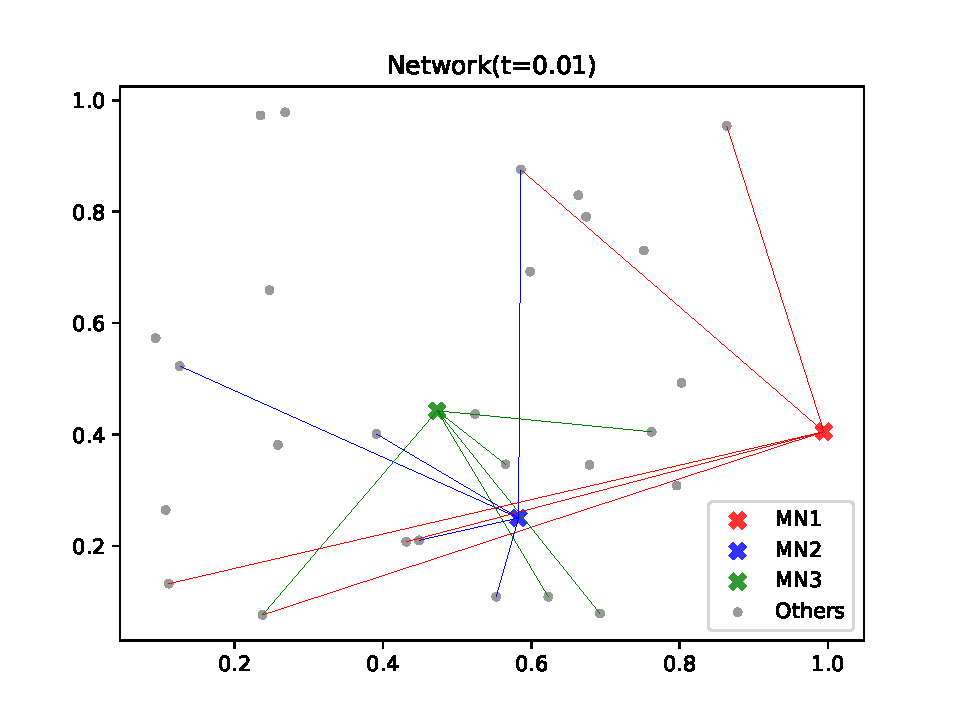
\includegraphics[width = 0.3\textwidth]{Graphs/t_001.pdf}
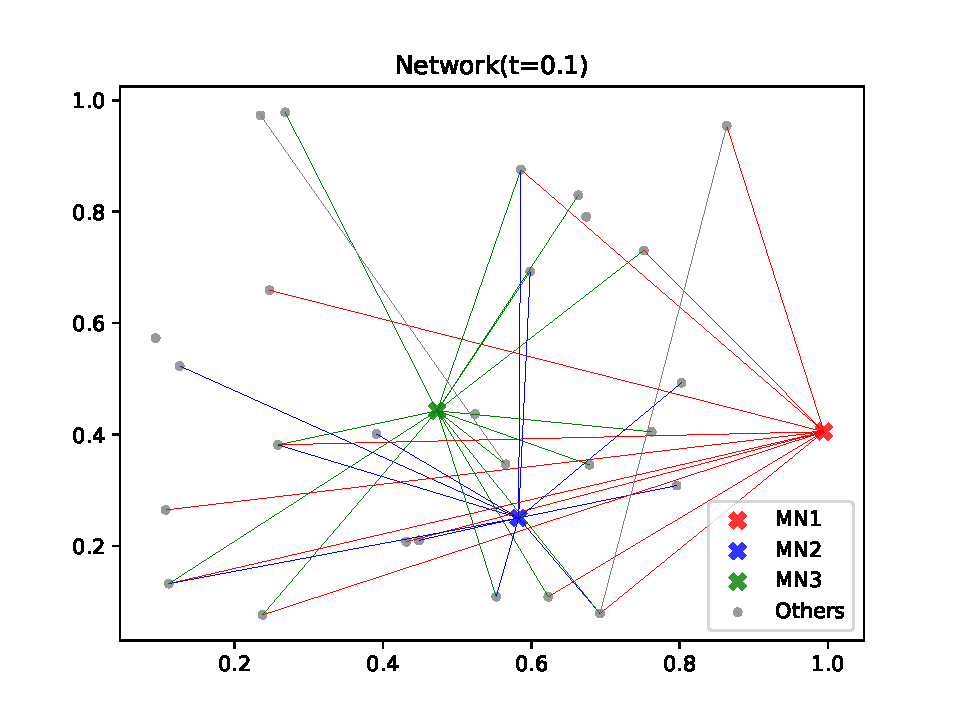
\includegraphics[width = 0.3\textwidth]{Graphs/t_01.pdf}
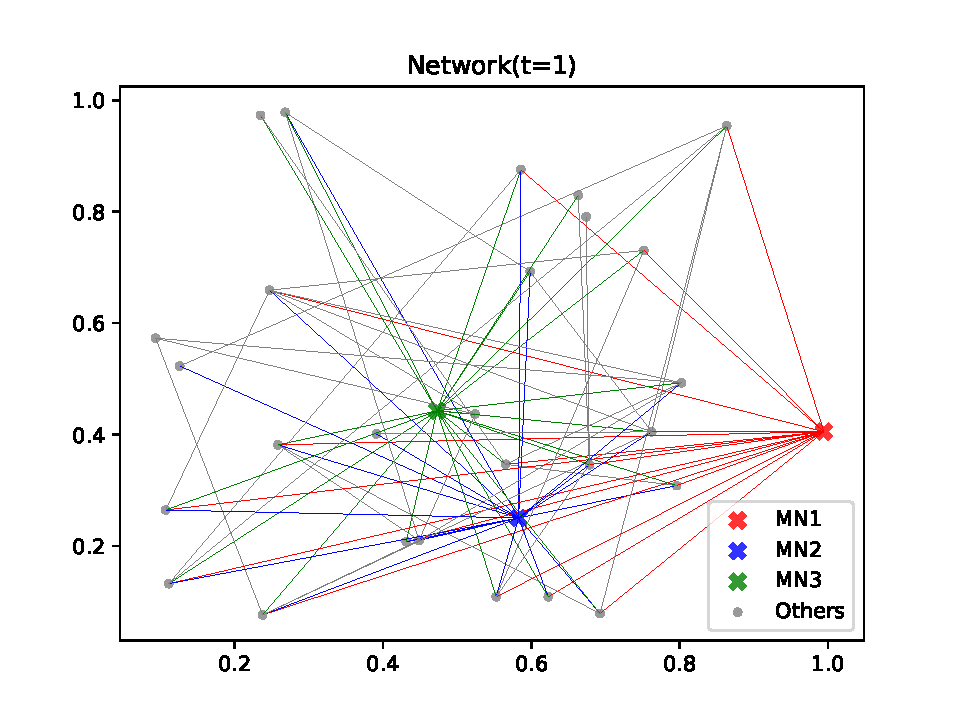
\includegraphics[width = 0.3\textwidth]{Graphs/t_1.pdf}\\
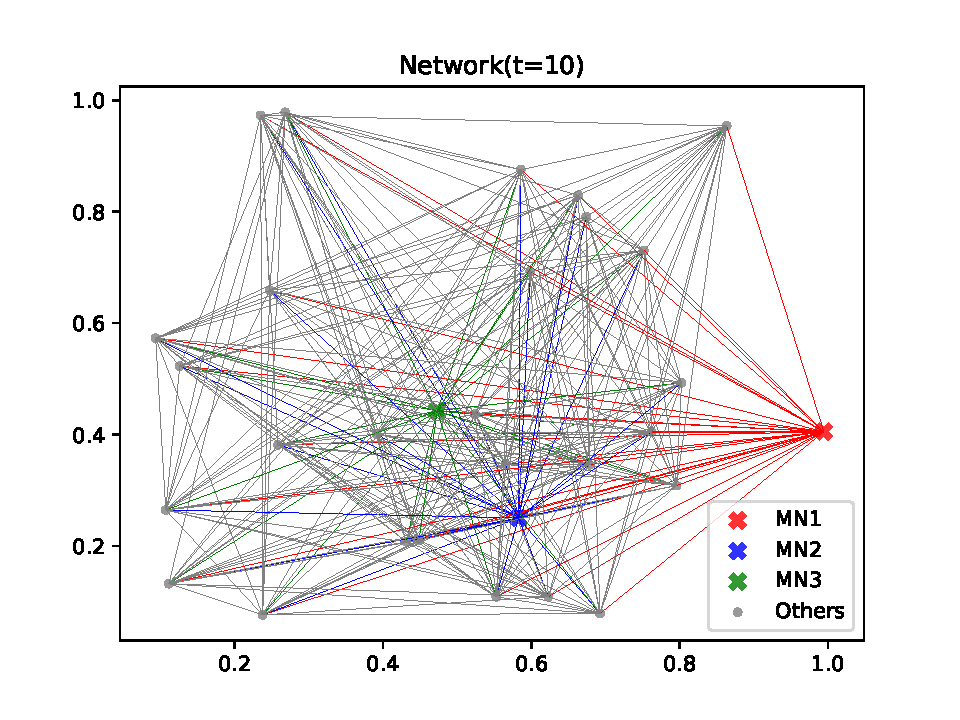
\includegraphics[width = 0.3\textwidth]{Graphs/t_10.pdf}
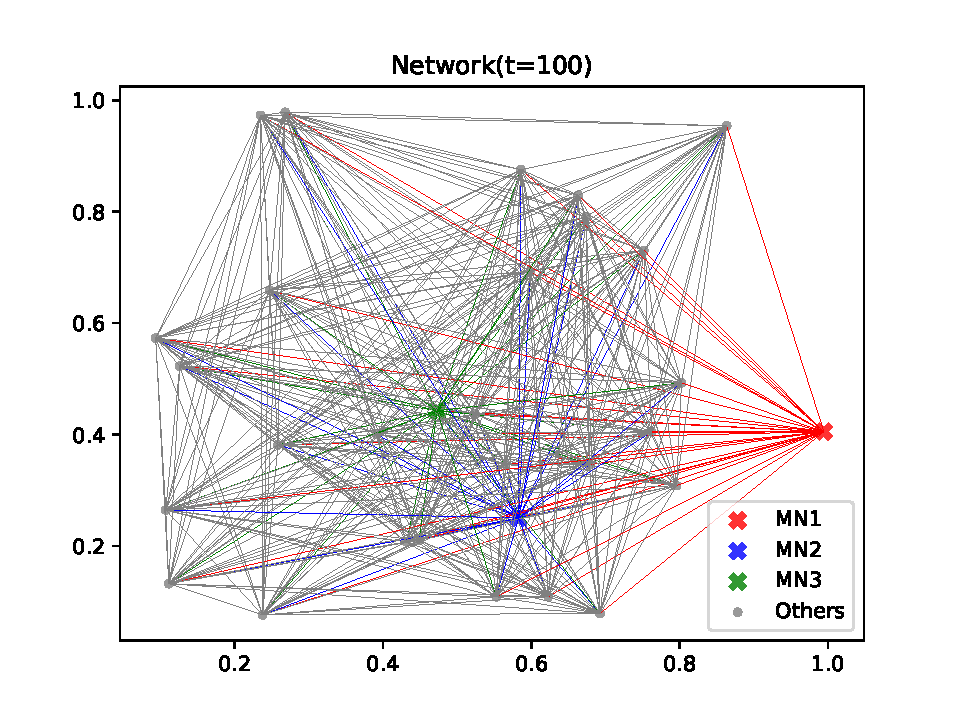
\includegraphics[width = 0.3\textwidth]{Graphs/t_100.pdf}
\caption{Development of the network with two cell types. The node $n_1$ is represented by ``MN1'' in red. The node $n_2$ is represented by ``MN2'' in blue. The node $n_3$ is represented by ``MN3'' in green. Other nodes are represented by ``Others'' in gray.}
\label{Fig: development of network}
\end{figure}
\noindent
Kernel method is used to estimate the intensity function (???) of each node based on the connecting time points. 
Cross-validation method is applied in order to choose the optimal bandwidth.
\\
The $\ell_2$-distance is adopted as a measure of dissimilarity between the estimated intensity functions.
The hierarchical clustering is then used to cluster nodes based on the pairwise $\ell_2$-distances. Specifically, the average distance is used as the distance between two sets.
\\
It turns out that $\mathbf{G}_1$ and $\mathbf{G}_3$ are clustered completely correct, whereas in $\mathbf{G}_2$ only $n_3$ is recognized successfully among the three ``MNs''.
\\
To illustrate the reason, we plot the estimated intensity functions for each network (see Fig.\ref{Fig: fitted intensity functions}). It can be seen that the clusters of $\mathbf{G}_2$ are not distinct enough, which causes the failure to correctly cluster $n_1$ and $n_2$.
\begin{figure}[H]
\centering
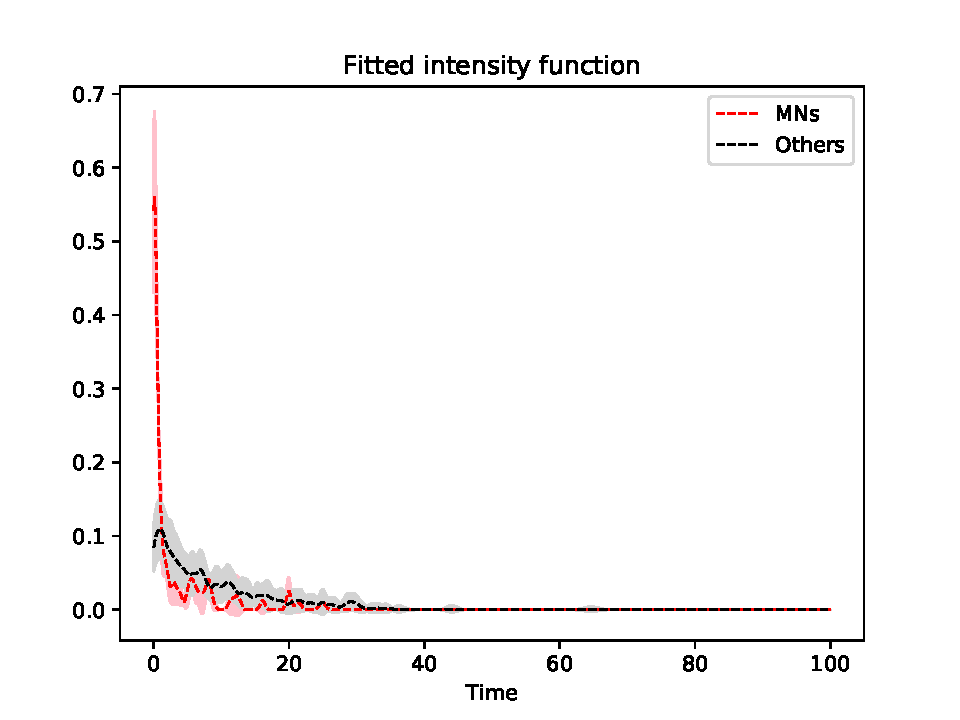
\includegraphics[width = 0.45\textwidth]{Graphs/fitted_intensity.pdf}
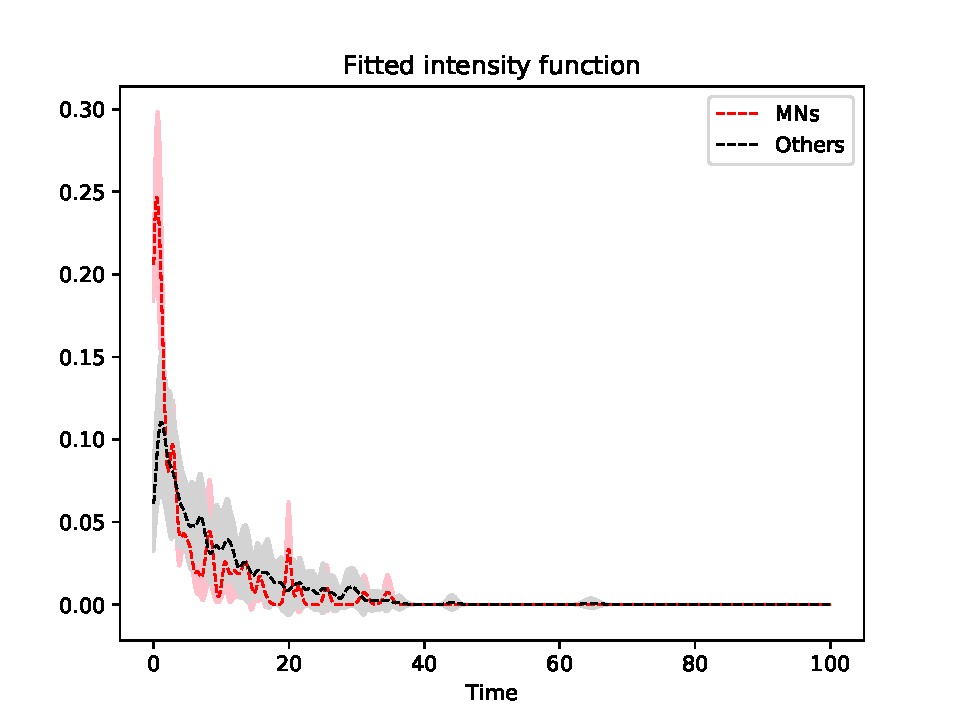
\includegraphics[width = 0.45\textwidth]{Graphs/fitted_intensity_alpha05_lamda01.pdf}
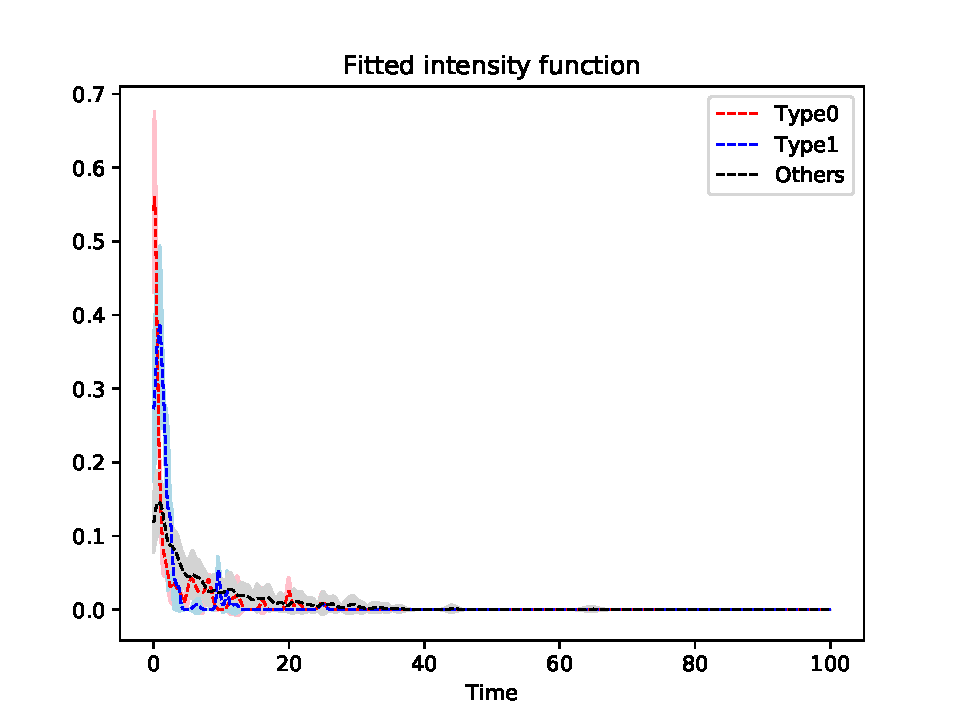
\includegraphics[width = 0.45\textwidth]{Graphs/fitted_intensity_three_types.pdf}
\caption{Fitted intensity functions. The top left figure corresponds to $\mathbf{G}_1$. The top right figure corresponds to $\mathbf{G}_2$. The bottom left figure corresponds to $\mathbf{G}_3$. The dashed lines represent the mean intensity of nodes in that cluster. The shaded area represents the standard deviations.}
\label{Fig: fitted intensity functions}
\end{figure}
